% CREATED BY DAVID FRISK, 2018
\chapter{Deep learning and Undertainty estimation}

According to \cite{rogers2016first}, Machine learning is an area in computer science were algorithms are used to simulate learning and infering. Most problems in machine learning can be boiled down to approximating the function that maps an input data $\bm{x}^{(\mu)}$ to it's correct target $\bm{t}^{(\mu)}$. Cases where to targets are known is called supervised learning and the cases where those are unknown are called unsupervised learning. In this thesis, we will be focusing on the task of classification which falls under supervised learning\cite{mehligcourseslides}.

Deep Learning is a field in the supervised learning branch of Machine learning where the Algorithms are learning from experience by performing the task over and over, and to stack each layer of information can extract on top of each other \cite{Goodfellow-et-al-2016}. In classic machine Learning, the input needs to be processed and filtered for the necessary information. This process is called feature engineering \cite{rogers2016first}. According to \cite{Goodfellow-et-al-2016}, by stacking the learnt information and experience, Deep learning based solutions mitigates this problem.

Today, most Deep Learning is accomplished using deep Artifical Neural Networks (ANN). The first part of this chapter will deal with the basics of deep learning, what are ANNs and how to train them. The second part of this chapter will be presenting the scheme proposed by Lakshminarayanan et. al. \cite{lakshminarayanan2017simple} involving deep neural network ensembles. The last section will deal with the metric we will use in this thesis. This includes classification error, accuracy, and information entropy. 

\section{Artificial Neural Networks}

\begin{figure}
    \centering
    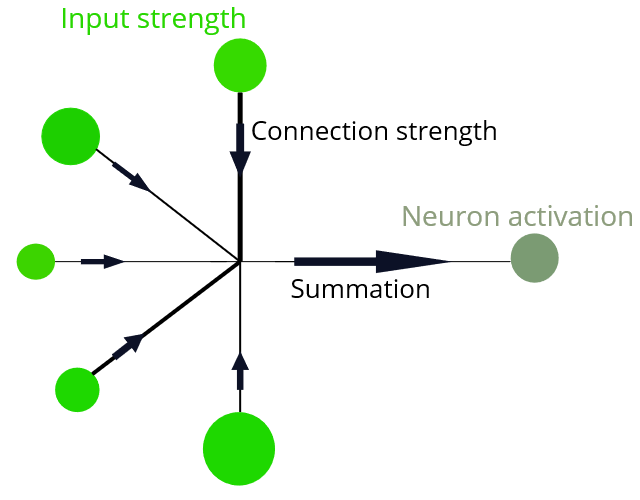
\includegraphics[scale=0.5]{figure/neuron_activation.png}
    \caption{Illustration of the activation process of McCulloch Pitts Neurons. Original figure created by \cite{barkdeep}}
    \label{fig:mcculloch-pitts}
\end{figure}

Neural networks are mathematical models inspired by the interaction between the neurons in the brain\cite{mehligcourseslides,Goodfellow-et-al-2016}. A neuron unit receives the input signals from neighboring neurons and gives an output. In Machine learning, Neural networks referes to models that uses the Neuron synapse model proposed by Warren McCulloch and Walter Pitts\cite{McCulloch1943,hopfield1984neurons}.

Consider a neuron unit $j$ which are connected to $i$ neurons, \cite{McCulloch1943} models the output synapse $v_j$ of neuron $j$ using equation \eqref{eq:mcculloch}. Here, $v_i$ represents the incoming synapses from the $i$ connected neurons, $W_{ij}$ represents the connection strength between neuron $i$ and $j$, the function $g(.)$ is called an activation function, and $\theta_j$ represents the activation threshold (this is known as the Bias term in some literature\cite{Goodfellow-et-al-2016}).

\begin{equation}
    \label{eq:mcculloch}
    v_j = g\left(\sum_i W_{ij} v_i - \theta_j\right)
\end{equation}

Figure \ref{fig:mcculloch-pitts} is a simple caricature representation of the model described in equation \eqref{eq:mcculloch}.

\begin{figure}
    \centering
    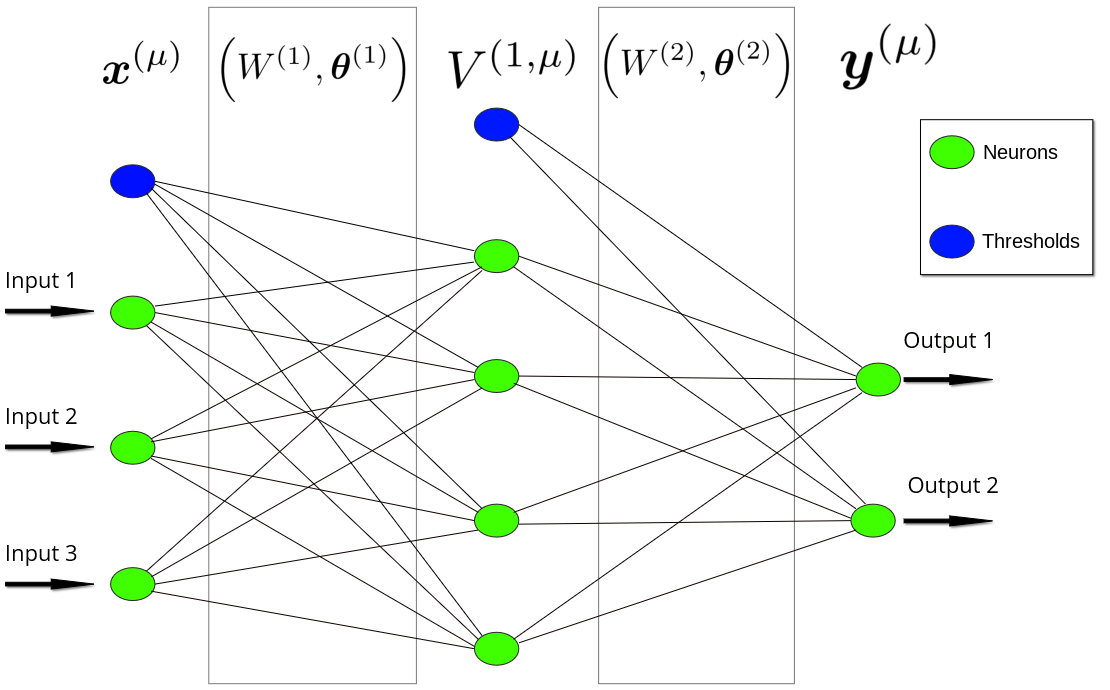
\includegraphics[scale=1.3]{figure/neural_network1.png}
    \caption{Illustration of a Multilayer Perceptron. This figure can be found in \cite{barkdeep}. Minor modifications have been applied to the original in order to better fit it into this report}
    \label{fig:mlp}
\end{figure}

\subsection{Multi-Layer Perceptrons and Fully connected layers}

Suppose that we are to model the output of several neurons, let $\boldsymbol{v}_n$ denote the vector that represents the activation of $n$ neurons. A consequence of \eqref{eq:mcculloch} is that this output can be modelled using linear algebra as according to equation \eqref{eq:linalgmcculloch}. Here the weights $W$ is a $n \times m$ matrix that represents the connection between the $n$ neurons and $m$ others and $\boldsymbol{v}_m$ is the incoming singal from the $m$ neurons\cite{mehligcourseslides}. 

\begin{equation}
    \label{eq:linalgmcculloch}
    \boldsymbol{v}_n = g(W\boldsymbol{v}_m-\boldsymbol{\theta_n})
\end{equation}

In deep learning, several McCulloch Pitts neurons are wired together in a layer by layer structure using equation \eqref{eq:linalgmcculloch}. These networks consist of an input layer and an output layer. Between input and output, there could exists a number of hidden layers. Such a network are known as a multi-layer perceptrons(MLPs)\cite{mehligcourseslides}, an illustrated example with one hidden layer can be seen in figure \ref{fig:mlp}.

Suppose that we are to feed the $n$ dimensional input pattern $\boldsymbol{x}^{(\mu)}$ through an MLP similar to the one illustrated in figure \ref{fig:mlp}. The states $V_j^{(1,\mu)}$ for neuron $j$ in the hidden layer of the $m$ neurons are calculated using equation \eqref{eq:hidden1}.

\begin{equation}
    \label{eq:hidden1}
    V^{(1,\mu)}_j = g\left(\sum_{i=1}^nW^{(1)}_{ij} x^{(\mu)}_i - \theta^{(1)}_j\right)
\end{equation}

The outputs $y_k^{(\mu)}$ from this network can than be calculated as a function of the neuron synapses $V^{(1,\mu)}_j$ from the hidden layers by equation \eqref{eq:output}

\begin{equation}
    \label{eq:output}
    y_k^{(\mu)} = f\left(\sum_{j = 1}^m W_{jk}^{(2)}V_j^{(1,\mu)} - \theta^{(2)}_k\right)
\end{equation}

In the case were there are $L$ hidden layers instead of just 1, than the output calculation is still calculated in the same way as in equation \eqref{eq:output}, and each of neuron activation $V^{(\ell,\mu)}_j$ in any hidden layer $\ell$ are calculated in terms of the previous layer $\ell-1$ according to \eqref{eq:hidden}

\begin{equation}
    \label{eq:hidden}
    V_j^{(\ell,\mu)} = g\left(\sum_{i}W^{(\ell)}_{ij} V^{(\ell-1,\mu)}_i-\theta^{(\ell)}_j\right) 
\end{equation}

A layer where all neurons are connected to every neuron in the previous layers are known as a \textit{Fully connected layer}\cite{Goodfellow-et-al-2016}, in some literature, these are known as dense layers\cite{chollet2018deep}.

\subsection{Convolutional Neural Networks}

According to \cite{Goodfellow-et-al-2016}, Convolutional Neural Networks (CNNs) are ANNs designed to work with inputs that have a grid-like topology, such as 2D images. While regular fully connected dense layers makes use of matrix multiplication. CNN uses a variation of \textit{discrete convolution}\cite{Goodfellow-et-al-2016}. Convolution is an operation between two functions of same dimensionality and is defined in eq. \eqref{eq:convolution}

\begin{equation}
    \label{eq:convolution}
    s(t) = (x * w)(t) = \sum_a x(a)w(t-a)
\end{equation}

In neural networks, the first argument $x$ of \eqref{eq:convolution} is refered to as the input, and the second argument $w$ is called the kernel. usually, the input is an multidimensional array (a.k.a a Tensor), and the kernel is a multidimensional array of parameters. Convolution is also an operation that is conveniently defined on multiple axis. Suppose that the input is a two dimensional image $X^{(\mu)}$, then the kernel $W^{(1)}$ also have to be two dimensional. A consequence of this is that the output will also be multidimensional, with the activation $V^{(1,\mu)}_{ij}$ for neuron $(i,j)$ in this convolutional layer calculated as according to eq. \eqref{eq:convneuron}. Here $g(.)$ denotes an activation function. In context of convolutional neural networks, $V^{(1,\mu)}_{ij}$ is also refered to as a \textit{feature map}\cite{mehligcourseslides}.

\begin{equation}
    \label{eq:convneuron}
    V^{(1,\mu)}_{ij} = g\left[(X^{(\mu)} * W^{(1)})(i,j)\right] = g\left[\sum_m\sum_n X^{(\mu)}_{i+m,j+n} W^{(1)}_{mn}\right]
\end{equation}

Do note the change of sign in the denominator in \eqref{eq:convneuron} vs \eqref{eq:convolution}. This is because the formula in \eqref{eq:convneuron} is an alternative form for writing convolution that is more widely used when implementing CNNs\cite{Goodfellow-et-al-2016}. In most cases, the kernals are smaller ins size compared to the input, thus some literature describes them as filter that scans and performs the convolution operation in eq. \eqref{eq:convneuron} on smaller parts of the input at a time. Figure \ref{fig:convolution} illustrate the convolution operations that occures in a CNN.

\begin{figure}
    \centering
    \includegraphics[scale=0.5]{figure/convolution.png}
    \caption{Illustration of convolution in CNNs. Given a $3\time3$ input, using a Kernel of size $2\times 2$, the feature maps are calculated according to the formulas in the figure. Origianl figure can be found in \cite{barkdeep}, based of the figure used by \cite{Goodfellow-et-al-2016}}
    \label{fig:convolution}
\end{figure}

Additionally, the outputs from convolutional layers also filtered through a so called Pooling layer. The neurons of a Pooling layer takes the output from it's connected feature maps and summerises them to a single number. Examples of pooling layers includes the MaxPooling layer which outputs the maximum of it's connected feature maps, and L2-Pooling layer computes the Root-Mean-Square value of the featuer map outputs\cite{mehligcourseslides}.

\section{Classification Problems}

Already previously, we described most Machine Learning problems to be approximating the function that maps a given input $\bm{x}^{(\mu)}$ to it's correct target $\bm{t}^{(\mu)}$. In classification problems involving $N$ different labels\footnote{Sometimes known as it's class, hence, the name classification problems}, than each input $\bm{x}^{(\mu)}$ are to be assigned it's target $\bm{t}^{(\mu)}$. Here $\bm{t}^{(\mu)}$ will be a representation of the correct integer class $c^{(\mu)}$ of pattern $\bm{x}^{(\mu)}$. 

An approach to classification problems in ML is to approximate the discrete probability distribution of the conditional probability $y_i^{(\mu)} = P(c = i | \bm{x}^{(\mu)})$ such that $y_i^{(\mu)}$ is largest when $i$ corresponds to the correct class $c^{(\mu)}$, and smaller otherwise. A machine learning model that uses this prediction scheme is called a probabilistic classifier \cite{rogers2016first}.

To create and train probabilistic classifiers, the targets $\bm{t}^{(\mu)}$ needs to be encoded as $N$ dimensional one hot vector by eq \eqref{eq:target1hot} \cite{mehligcourseslides}.

\begin{equation}
    \label{eq:target1hot}
    t_i^{(\mu)} = 
    \begin{cases}
        1 & \text{if } i = c^{(\mu)}\\
        0 & \text{otherwise}
    \end{cases}
\end{equation}

Once the classifier is trained, the algorithm assigns the class $\hat{c}^{(\mu)}$ to pattern $\bm{x}^{(\mu)}$ based on the output $\bm{y}^{(\mu)}$ from the trained model. This is done by computing the one-hot vector $\hat{\bm{t}}^{(\mu)}$ using eq. \eqref{eq:assign1hot}. In some cases, it is also acceptable to just compute $\hat{c} = \argmax_i \bm{y}^{(\mu)}$, this is nothing we do in this thesis.

\begin{equation}
    \label{eq:assign1hot}
    \hat{t}_i^{(\mu)} = \begin{cases}
        1 & \text{if }i = \argmax_i \bm{y}^{(\mu)} \\
        0 & \text{otherwise}
    \end{cases}
\end{equation}

According to \cite{mehligcourseslides} the output of a deep ANN can be transformed into probabilities by using the softmax activation function in the output layer. This function is defined in eq \eqref{eq:softmax}

\begin{equation}
    \label{eq:softmax}
    y_i = \frac{e^{\alpha b_i}}{\sum_{c = 1}^N e^{\alpha b_c}}
\end{equation}

Here $b_i$ stands for the local field of neuron $i$ in the output layer $b_i = \sum_j W_{ij}v_j - \theta_i$. The parameter $\alpha$ is usually set to unity ($\alpha = 1$). Apart from transforming the outputs of the ANN into probabilities, softmax also has the property that $y_i$ is largest when the synapses $b_i$ is the largest, and smaller otherwise. This is also the property that ensures that the ANNs can be used as probabilistic classifiers.

\section{Training the Neural Network}
\label{sect:train}

In order for an ANN to correctly predict the label of an input pattern $\bm{x}^{(\mu)}$, correct the weights $W^{(l)}$ and thresholds $\bm{\theta}^{(l)}$ are required. The question remains, how do we set the correct weights and thresholds?

Given a classification problem $\{(\bm{x}_T^{(\mu)},\bm{t}_T^{(\mu)})| \mu = 1,...,P\}$ with $P$ training samples. The problem of finding the correct weights can be viewed as an optimization problem where the parameters are adjusted iteratively to minimize a loss function, also known as the \textit{Energy Function} \cite{mehligcourseslides,Goodfellow-et-al-2016}. For each iteration, the paramters are updated using \textit{gradient descent}.

\subsection{Energy Functions}
\label{sect:energyfunc}
An energy function $H$ is a function that are defined in terms of the inputs, targets, and the parameters of the ANN model. For classification problem, the function $H$ needs to fulfill these properties:

\begin{enumerate}
    \item $H$ has to be differentiable with respect to the parameters in the ANN.
    \item $H$ gets smaller when the classification error (probability of an ANN making an incorrect prediction) gets smaller.
\end{enumerate}

The first rule is needed since it allows us to update any parameter $W$ in the ANN using the gradient descent update rule defined in \eqref{eq:update}. The parameter $\eta$ in \eqref{eq:update} is the step length. In context of ANN training $\eta$ is also called the learning rate.

\begin{equation}
    \label{eq:update}
    W^{(t+1)} = W^{(t)} - \eta \frac{\partial H}{\partial W}
\end{equation}

The second property ensures that the classification of the ANN goes down as we adjust the parameters of the network to minimize the energy function. According to \cite{mehligcourseslides,lakshminarayanan2017simple,quinonero2006evaluating}, the negative log-likelihood in eq. \eqref{eq:nll} is the preferred energy function when training probabilistic ANN classifiers. Negative Log-likelihood is also known as the Cross-Entropy loss function \cite{quinonero2006evaluating}.

\begin{equation}
    \label{eq:nll}
    H = -\sum_{\mu}\sum_it_i^{(\mu)}\log_2y_i^{(\mu)}
\end{equation}

\subsection{Backpropagation}

\label{sect:backprop}

The procedure of finding the gradients of the energy function with respect to the network parameters are known as backpropagation \cite{lecun1988theoretical}. 
Suppose that we have a Multilayere Perceptron with $L$ hidden layers, given pattern $\bm{x}^{(\mu)}$, the neuron state update rules in each of the layers would be that of \eqref{eq:feed1},\eqref{eq:feed2} and \eqref{eq:feed3}.

\begin{align}
    V^{(\ell,\mu)}_j = g(b_j^{(\ell,\mu)}) && b_j^{(\ell,\mu)} = \sum_i W^{(\ell)}_{ij}x^{(\mu)}_i - \theta_j^{(\ell)}&&\ell = 1\label{eq:feed1}\\
    V^{(\ell,\mu)}_k = g(b_k^{(\ell,\mu)}) && b_k^{(\ell,\mu)} = \sum_j W^{(\ell)}_{jk}V_j^{(\ell-1,\mu)} - \theta^{(\ell)}_k && 1 < \ell < L \label{eq:feed2}\\
    y_l^{(\mu)} = f(b_l^{(O,\mu)}) && b_l^{(O,\mu)} = \sum_k W^{(O)}_{kl}V_k^{(\ell,\mu)}-\theta^{(O)}_l && \ell = L \label{eq:feed3}
\end{align}

To calculate the update gradient $\dfrac{\partial H}{\partial W^{(O)}_{mn}}$ for the weights $W^{(O)}_{mn}$ that connects layer L to the output layer, we will differentiate the energy function $H$ by using the chain rule in the fashion of \eqref{eq:backprop1} where $\frac{\partial H}{\partial y^{(\mu)}_i}$ is the derivative of the energy function w.r.t. to neuron $y^{(\mu)}_i$, $\frac{dy_i^{(\mu)}}{db^{(L,\mu)}_i}$ is the derivative of the output w.r.t. to it's localfield, and finally, $\frac{db_i^{(L,\mu)}}{dW^{(L)}_{mn}}$ is the derivative of the localfield w.r.t. the weight $W^{(L)}_{mn}$.

\begin{equation}
    \label{eq:backprop1}
    \frac{\partial H}{\partial W_{mn}^{(O)}} = \frac{\partial H}{\partial y^{(\mu)}_m}\frac{dy_m^{(\mu)}}{db^{(O,\mu)}_m}\frac{db_m^{(O,\mu)}}{dW^{(L)}_{mn}}
\end{equation}

Using the equations \eqref{eq:feed1},\eqref{eq:feed2} and \eqref{eq:feed3},We can decompose each of the derivatives in \eqref{eq:backprop1} into \eqref{eq:deriv1} and \eqref{eq:deriv2}. Here $f'(.)$ is the derivative of the activation function $f$ of the output layer.

\begin{align}
    \frac{dy_m}{db_m} = f'(b_m)\label{eq:deriv1} \\
    \frac{db_m}{dW_{mn}} = V_n \label{eq:deriv2}
\end{align}

Inserting \eqref{eq:deriv1} and \eqref{eq:deriv2} into \eqref{eq:backprop1}, the final equation for calculating the gradients with respect to the weight becomes eq \eqref{eq:backprop12}.

\begin{equation}
    \label{eq:backprop12}
    \frac{\partial H}{\partial W_{mn}^{(O)}} = \frac{\partial H}{\partial y_m^{(\mu)}}f'(b_m)V^{(L,\mu)}_n = \Delta_E^{(O,\mu)}V^{(L,\mu)}_n
\end{equation}

A consequence of the equations for the localfield, differentiating the localfield w.r.t. thresholds would always be $-1$. Thus the update gradient for the thresholds becomes \eqref{eq:backprop13}.

\begin{equation}
    \label{eq:backprop13}
    \frac{\partial H}{\partial \theta^{(O)}_m} = \frac{\partial H}{\partial y_m^{(\mu)}}f'(b_m)(-1) = -\Delta_E^{(O)}
\end{equation}

Next, the weights between layer $L$ and $\ell = L-1$ are to be updated. The gradients for the weights are obtained by continuing applying the chain rule\cite{mehligcourseslides}. However, as a consequence of how localfield $b^{(O,\mu)}_l$ is calculated (see eq \eqref{eq:feed3} and \eqref{eq:feed2}), the weights $W^{(L)}_{mn}$ appears in all of the terms of $V_k^{(L,\mu)}$, thus the partial derivatives $\frac{\partial b_l^{(O,\mu)}}{\partial W^{(\ell)}_{mn}}$ needs to be summed. This is done using equation \eqref{eq:backprop2},\eqref{eq:backprop21} and \eqref{eq:backprop22}.

\begin{align}
    \frac{\partial H}{\partial W^{(L)}_{mn}}=\frac{\partial H}{\partial y^{(\mu)}_l}\frac{dy_l^{(\mu)}}{db^{(O,\mu)}_l}\frac{db_l^{(O,\mu)}}{dW^{(L)}_{mn}} && \label{eq:backprop2}\\
    \frac{\partial b^{(O,\mu)}_l}{\partial W^{(L)}_{mn}} = \sum_k W^{(O)}_{kl} \frac{dV_k^{(L,\mu)}}{dW^{(L)}_{mn}}  &&\label{eq:backprop21}\\
    \frac{\partial V_k^{(L,\mu)}}{\partial W^{(L)}_{mn}} = \frac{\partial V_k^{(L,\mu)}}{\partial b_k^{(L,\mu)}}\frac{db_k^{(L,\mu)}}{dW^{(L)}_{mn}} = g'(b_k^{(L,\mu)})\delta_{km}V^{(\ell,\mu)}_n  &&\label{eq:backprop22}
\end{align}

The factor $\delta_{km}$ denotes the kronecker delta, which is a function that takes the value of 1 when $k=m$, otherwise it takes the value of 0. Similarly, to get into the next hidden layer, we reapply the chain rule to find the update gradient for the weights and threshold in that layer. This is possible due to the layered structure of multi layer perceptrons \cite{mehligcourseslides}. Once the gradients for the layers are computer, the weights and thresholds are updated according to equation \eqref{eq:update}. A direct implication of eq \eqref{eq:deriv1} and \eqref{eq:backprop22} is that the activation functions also needs to be differentiable.

\subsection{Stochastic Gradient Descent and Mini Batch}

\begin{figure}
    \centering
    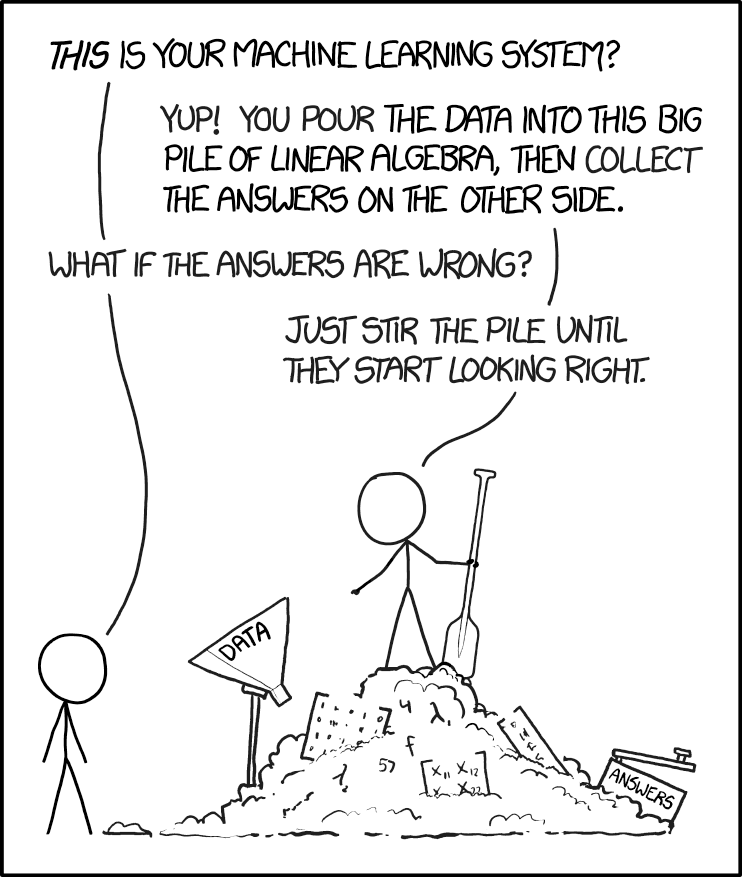
\includegraphics[scale=0.3]{figure/machine_learning_2x.png}
    \caption{A satirical, but very informative description of machine learning. Original image from XKCD, index: 1838. This image can be found at \cite{xkcd1838}}
    \label{fig:xkcd1838}
\end{figure}

In order to find the correct weights and thresholds for Deep ANNs, in iterative process that uses gradient descent is used to update the weights. The gradients are calculated using error backpropagation described in section \ref{sect:backprop}.

In the beginning weights and thresholds are initialized using a standard gaussian distribution \cite{mehligcourseslides}. Training samples $\bm{x}^{(\mu)}_T$ are then fed through the network. Using an energy function $H$, the update gradients of the weights and thresholds in each layer is calculated by applying chain rule error backpropagation. The parameters of the ANN is then updated using eq \eqref{eq:update}. Albeit satirical, figure \ref{fig:xkcd1838} works as a summery of the process of training Deep ANNs.

As the energy function $H$ isn't necessarily convex in the space of the weights and thresholds \cite{kingma2014adam}, some stochastic methods are used to mitigate the possibilities of the training to converge while only finding a local optima in $H$ w.r.t. to the ANN parameters. One of these is to use a stochastic gradient descent algorithm where the training samples are either sampled one by one, or by simply just shuffling the order the training samples are fed through the network \cite{mehligcourseslides}. In most cases, this algorithm minimizes the risk of the weights getting stuck on saddle points, and local optimums \cite{lecun2015deep}.

According to \cite{mehligcourseslides} it is also possible to feed all of the training samples in one go through the network. This is called batch training. A drawback of this method is that the network parameters runs a greater risk of getting stuck at a local minimum of the energy function due to the more deterministic trajectory through the parameter space of the energy function, especially if the training samples are not randomly permuted between iterations.

A middle ground between batch and full stochastic gradient descent is the use of mini-batches. The training samples are randomly permuted and divided into mini-batches of size $m_B$. The energy function are then normalize across the minibatch. According to \cite{mehligcourseslides}, this can greatly speed up the training while still mitigating the risk of the parameters to converge onto a local minimum.

Stochastic Gradient Descent can be augmented using adaptive learning rate with regulated momentum depending on the gradient norm. Doing this results in an optimization algorthim known as \textit{Adam}\cite{kingma2014adam}.

\section{Scheme for Estimating Predictive Uncertainty}
\label{sect:uncertainty}
This section will present the scheme for estimating the predictive uncertainty that was proposed by Lakshminarayanan et. al. at deep mind \cite{lakshminarayanan2017simple}. Given a classification problem with $N$ labels and the set $T = \left\{(\bm{x}_T^{(\mu)},\bm{t}_T^{(\mu)}) | \mu = 1,...,P\right\}$ with $P$ training samples and corresponding targets. The scheme proposed by \cite{lakshminarayanan2017simple} consist of the following three components
\begin{enumerate}
    \item Choosing a proper scoring rule as training criterion.
    \item Use \textit{adversarial training} to smooth the predictive distribution.
    \item Train an \textit{ensemble}
\end{enumerate}

These three components are described in detail in the following subsections.

\subsection{Proper scoring rule}

\cite{lakshminarayanan2017simple} described a proper scoring rule as a function that rewards better calibrated predictions over worse. While this is similar to the properties of energy functions listed in sect. \ref{sect:energyfunc}, a scoring function $S$ assign higher values to better calibrated predictions instead of lower. 

Suppose that $S(\bm{y}^{(\mu)},(\bm{x}^{(\mu)},\bm{t}^{(\mu)}))$ is a scoring rule that evaluates the predictive distribution made by an ANN $y_i^{(\mu)} = p\left(c = i|\bm{x}^{(\mu)}\right)$. In probabilistic classifiers, $c$ denotes the class of which we are looking to assign input $\bm{x}^{(\mu)}$. Most importantly, $S$ needs to satisfy \eqref{eq:scorerule1} and the equivalence implication in \eqref{eq:scorerule2}

\begin{equation}
    \label{eq:scorerule1}
    S[\bm{y}^{(\mu)},(\bm{x}^{(\mu)},\bm{t}^{(\mu)})] \leq S[\bm{t}^{(\mu)},(\bm{x}^{(\mu)},\bm{t}^{(\mu)})]
\end{equation}

\begin{equation}
    \label{eq:scorerule2}
    S[\bm{y}^{(\mu)},(\bm{x}^{(\mu)},\bm{t}^{(\mu)})] = S[\bm{t}^{(\mu)},(\bm{x}^{(\mu)},\bm{t}^{(\mu)})] \iff \bm{y}^{(\mu)} = \bm{t}^{(\mu)}
\end{equation}

ANNs are then trained using the energy function $H = -S$

According to \cite{lakshminarayanan2017simple}, many common energy functions used for training neural networks fulfills the property required for a proper scoring rule, including the negative log-likelihood function in \eqref{eq:nll} that are used when training ANN as a probabilistic classifier.

\subsection{Adversarial training}
\label{sect:adv}
Adversarial examples are datapoints that are special engineered to trick a machine learning algorithm into making an incorrect decision\cite{nguyen2015deep,lowd2005adversarial} Given an arbitary input pattern $\bm{x}^{(\mu)}$ and an energy function $H$, an efficient way of generating the adversarial example $\bm{x}'^{(\mu)}$ is described in eq. \eqref{eq:fgs}. This method is known as the fast gradient sign method and was designed by \cite{goodfellow2014generative}.

\begin{equation}
    \label{eq:fgs} 
    \bm{x}'^{(\mu)} = \bm{x}^{(\mu)} + \epsilon \text{sign}({\nabla_{\bm{x}^{(\mu)}}H})
\end{equation}

The idea behind adversarial training(AT) is to generate adversarial examples during training and than treated as additional samples in the training set \cite{goodfellow2014generative}. This is done by generating the adversarial example $\bm{x}'^{(\mu)}$ (using for instance \eqref{eq:fgs}) for each given input $\bm{x}^{(\mu)}$, and then perform the gradient descent procedure with error backpropagation using the generated $\bm{x}'^{(\mu)}$ as input to the network.

According to \cite{goodfellow2014generative}, training a Machine Lerning algorithm this way results in improved robustness of the classifier. Lakshminarayanan et. al. \cite{lakshminarayanan2017simple} also states that AT smooths the predictive distributions.

\subsection{Ensembles: training and predictions}

In machine learning, ensemble training refers to model that combines multiple machine learning algorithms to produce better results \cite{lee2015m}. In deep ensemble refers to ensembles consisting of deep ANNs.

In general there are two ways of training an ensemble. One is randomization methods were each models can be trained independently of each other, and one is the use of boosting, where the ensemble members are trained sequentially\cite{zhou2002ensembling}. In this thesis, we will mainly be focusing on randomization methods since this is the training model used by \cite{lakshminarayanan2017simple}. Another motivation for the use of randomization over boosting is that it enables us to train each ensemble member independent of each other, which means that they can be trained in an independent manor.

Given an ensemble size $K$, the training scheme use by Lakshminaryanan et. al. \cite{lakshminarayanan2017simple} can be boiled down to these steps

\begin{enumerate}
    \item Initialize each of the $K$ members weights and thresholds independently.
    \item Each member are than given the whole training set shuffled randomly.
    \item Train each of the ensemble members using their shuffled training samples as input.
    \item Alternative to 3), use adversarial training described in sect \ref{sect:adv}.
\end{enumerate}

Another way of training randomization ensembles is to use bagging (or bootstrapping) where each members are only given their own subset of the training data \cite{breiman2001random}. We will favor the training procedure used by \cite{lakshminarayanan2017simple} due to it outperforming bagging methods according to \cite{lee2015m,lakshminarayanan2017simple}.

Training aside, there exist a numerous way of modelling the prediction made by an ensemble \cite{lee2015m,li2018research,zhou2002ensembling}. Suppose that we have an ensemble of size $K$, with $\bm{y}^{(k)}$ being the output of member $k$, then one way of modeling the ensemble prediction $\bm{Y}^{(K)}$ is to average the predictions made be each member using equation \eqref{eq:avgensemble}

\begin{equation}
    \label{eq:avgensemble}
    Y^{(K)}_i = \langle y^{(k)}_i \rangle = \frac{1}{K}\sum_{k=i}^K y^{(k)}_i
\end{equation}

In their work, Lakshminaryanan et. al. \cite{lakshminarayanan2017simple} modelled the ensemble output using the averaging model in \eqref{eq:avgensemble}.
According to \cite{zhou2002ensembling}, this scheme is more favored when facing regression problems. Zhou et. al. \cite{zhou2002ensembling} and Hansen et. al. \cite{hansen1990neural} both suggested that a prediction scheme more resembling the a voting system is better for classification problems. Hansen et. al. \cite{hansen1990neural} described a vote by member $k$ to be the one hot vector $\hat{\bm{t}}^{(k)}$ computed using \eqref{eq:assign1hot}, then the ensemble prediction $\bm{Y}^{(K)}$ will be \eqref{eq:voteensemble}
\begin{equation}
    \label{eq:voteensemble}
    Y^{(K)}_i = \frac{1}{K}\sum_{k=1}^{K} \hat{t}^{(k)}_i
\end{equation}

In this thesis, both ensembles using averaging and voting are used to compare their impact with regards to performance and predictive uncertainty estimation.

\section{Scoring metrics}
\label{sect:scoring}
In this thesis, we will mainly be focusing on two different metric that are used to evaluate the scheme for estimating predictive uncertainty in neural network ensembles. In this thesis, we will mainly be using information entropy to measure the predictive uncertainty. We also measures the classification error made by the different ANN models. This is done in order to analyze the relation between entropy and classification error.

\subsection{Information Entropy}

Information entropy is a metric proposed by Claude Shannon \cite{jaynes1957information,shannon1948mathematical}. Let $X$ denote a discrete random variable with $N$ observable outcome with $P(X=i)$ denoting the probability to observe outcome $i$. Shannons formula for information entropy is stated according to eq \eqref{eq:entropy}.

\begin{equation}
    \label{eq:entropy}
    H(P(X)) = -\sum_{i=1}^N P(X=i)\log_2P(X=i)
\end{equation}

There are many ways of interpreting eq. \eqref{eq:entropy}. Shannon designed it as a function that can measure how certain we are of the outcome by observing the outcomes of $X$ \cite{shannon1948mathematical}. This is because \eqref{eq:entropy} has it's global maximum when $X$ is uniformly distributed (i.e. $P(X=i) = 1/N$) and is 0 when only one outcome is observable with unit probability. Essentially, information entropy is a function of the broadness of the distribution, which also falls under our intuitive understanding of uncertainty as we are more uncertain about an outcome when a distribution is broad, compared to a sharply peaked one \cite{jaynes1957information}. This is the main reason us to use entropy for measuring predictive uncertainty of Deep ANN predictions.

Suppose that $\bm{y}^{(\mu)}$ is the output from feeding the input pattern $\bm{x}^{(\mu)}$ through an ANN. The entropy of the network output $\bm{y}^{(\mu)}$ can than be calculated using eq. \eqref{eq:annentropy}.

\begin{equation}
    \label{eq:annentropy}
    H(\bm{y}^{(\mu)}) = -\sum_{i=1}^N y_i^{(\mu)}\log_2y_i^{(\mu)}
\end{equation}

\subsection{Classification Error}

Classification error represent the percentage of the input patterns that are incorrectly classified. Assuming a classification problem with $N$ labels,then the classification error can be calculated using eq. \eqref{eq:cerror} where the vector $\bm{\hat{t}}^{(\mu)}$ is the predicted target by the classifier that is calculated using \eqref{eq:assign1hot}\cite{mehligcourseslides}.

\begin{equation}
    \label{eq:cerror}
    C=\frac{1}{2p}\sum_{\mu=i}^{p}\sum_{i=1}^N|t_i^{(\mu)}-\hat{t}^{(\mu)}_i|
\end{equation}

Oppositing to classification error is classification accuracy, which stands for the percentage of the input patterns that are correctly classified. This implies that classification accuracy $C_{acc}$ can be calculated as $C_{acc} = 1 - C$\cite{mehligcourseslides}.
